\section{Results} \label{sec:results}

\begin{center}
\begin{tabular}{|c|c|c|}
\hline
\textbf{Parameter} & \textbf{Description} & \textbf{Value} \\ \hline
$n_r$ & Number of \emph{s-bots} & $50$ \\ \hline
$r_{rab}$ & Range and Bearning Range & $150$ [cm] \\ \hline
$n_s$ & Number of simulations & $50$ \\ \hline
$seed$ & Seed value for the simulation & \verb|$RANDOM|\footnotemark[1] \\ \hline
$tps$ & Simulation steps per second & 10 \\ \hline
\end{tabular}
\captionof{table}{Simulation parameters overview}
\label{tab:simparameters}
\end{center}
\footnotetext[1]{Internal function of the Bash shell. \url{http://tldp.org/LDP/abs/html/randomvar.html}}

\subsection{Metric definitions}\label{subsec:metric}
The developed method will be characterized by two metrics:
\begin{enumerate}
  \item Number of robots in chain (counted using the \verb|robot.in_chain| variable)
  \item Completion time (i.e. time needed to form a chain connecting  all the nest to all the 5 targets present in the environment).
\end{enumerate}
Since the strategy is mainly based on a random exploration, its performance can be regarded as a baseline value for comparison with more advanced methods.

\subsection{Communication range influence}\label{subsec:comrange}
The robots communicate among themselves by means of the Range and Bearing 
system, whose maximum range corresponds to $r_{rab}$ (cf. \ref{tab:simparameters}).

In the developed method, the main functions of this communication system are:
\begin{itemize}
  \item Attract the robots outside the nest (cf. \nameref{par:exitnest})
  \item Determine the attaching point to the chain (cf. \nameref{par:chainfollowing})
\end{itemize}

By reducing the communication range one would expect that:
\begin{itemize}
  \item An higher number of robots would be required to form the 
chain (since the robots would be closer to each other).
\item The process of exiting the nest would be slower (since less neighboring robots will be sensed).
\end{itemize}
Note that modification will affect the value of the chain distance parameter, for which the following inequality $d_{chain} < r_{rab}$ must hold. 
On the other hand, since the chain following behavior consists of a random walk, 
I believe that the reduction of the communication range would not affect this 
component of the behavior.

Unfortunately, an extensive study on the effect of the communication range, and thus the scalability of the method hasn't been performed within this project.

\subsection{Results distribution}
\begin{center}  
\begin{minipage}{.55\textwidth}
\begin{center}
\includegraphics[width=\textwidth,keepaspectratio]{{../Results/50Trials/Distributions}.pdf}

\vskip15pt
(a)
\vskip15pt


\end{center}
\end{minipage}%
\hspace{0.5cm}
\begin{minipage}{.35\textwidth}
\begin{footnotesize}
\begin{center}
\begin{tabular}{|l|c|c|}
\hline
& \multicolumn{1}{p{2cm}|}{\textbf{Robots in Chain}} & \multicolumn{1}{p{2cm}|}{\textbf{Completion Time}} \\
\hline
\textbf{Mean} &	36.82 & 21779.52 \\
\hline
\textbf{Std Dev} & 2.5689671 & 11138.0954867 \\
\hline
 \textbf{CV} = $\frac{\sigma}{\mu}$ & 0.06952743 &	0.51140223 \\
\hline
 \textbf{Median} & 37 &	21209.5 \\
\hline
\textbf{Min} & 30 & 6133 \\
\hline
\textbf{Max} & 41 & 47097 \\
\hline
\end{tabular}
\label{tab:summary}

\vskip15pt
(b)
\vskip15pt


\end{center}
\end{footnotesize}
\end{minipage}
\captionof{figure}{Panel containing the histograms and the empirical cumulative distribution functions for the designed metrics (a) with a summary of the relevant statistics of the two distributions (b)}
\end{center}

With the parameter settings shown in table \ref{tab:simparameters}, we can see that the number of robots required to connect the nest with the landmarks is bounded between a best-case value of $30$ and the worst-case value of $41$.
The range of the distribution of the \emph{Number of Robots} metric, is then higher than the 20\% of the overall number of robots $n_r$.

The variability of this results can be explained through several factors.

First of all, the random walk performed by the agents, even though slightly guided by the distance scanner, has no guarantee of either optimality, or determinism in the placement of the robots forming the chain.

By testing different values of the magnitude of the distance scanner force $\mathbf{F_{obs}}$ I noticed that there is a trade-off between the quality of the robot placement and the ability to reach the landmark.

In fact, higher values allow the robots to stop closer to the center of the corridors, but preventing them at the same time to go through the narrow passages that leads to the landmarks.

For this reason, the design choice was to focus on the reachability of the target positions, at the expense of a loss of positioning quality.

Furthermore, even though the landmarks could be reached, the spots can only be sensed if a robot is completely above it.
 
Sometimes, it may happen that a robot ignores the presence of the spot, even while being next to it, and tries to extend the chain in another direction, with respect to the target, thus increasing the number of robots in the chain.

Last but not least, the structure of the environment may yield to bifurcations of the chain, that yield in the end to the same target (that cannot be detected by the implemented algorithm), thus creating redundant branches that increase the number of required agents in the chain without actually bringing any benefits.

On the other hand, although approximately the 75\% of the trials are completed within 30000 simulation steps, there is a great variability in the time required to successfully complete the task, as shown by the variation coefficient (CV).

Given the nature of the method, the change in the value of the seed will affect only the initial position, initial orientation and the stopping position of the first robot (cf. \nameref{sec:sm}).

We can then conclude that the random change in the seed has a relevant impact on the completion time, while having a minor influence on the number of robots in the chain, that can be partially explained by the nature of the environment.

\subsection{Scatter-plot and correlation analysis}

\begin{center}  
\begin{minipage}{.55\textwidth}
\begin{center}
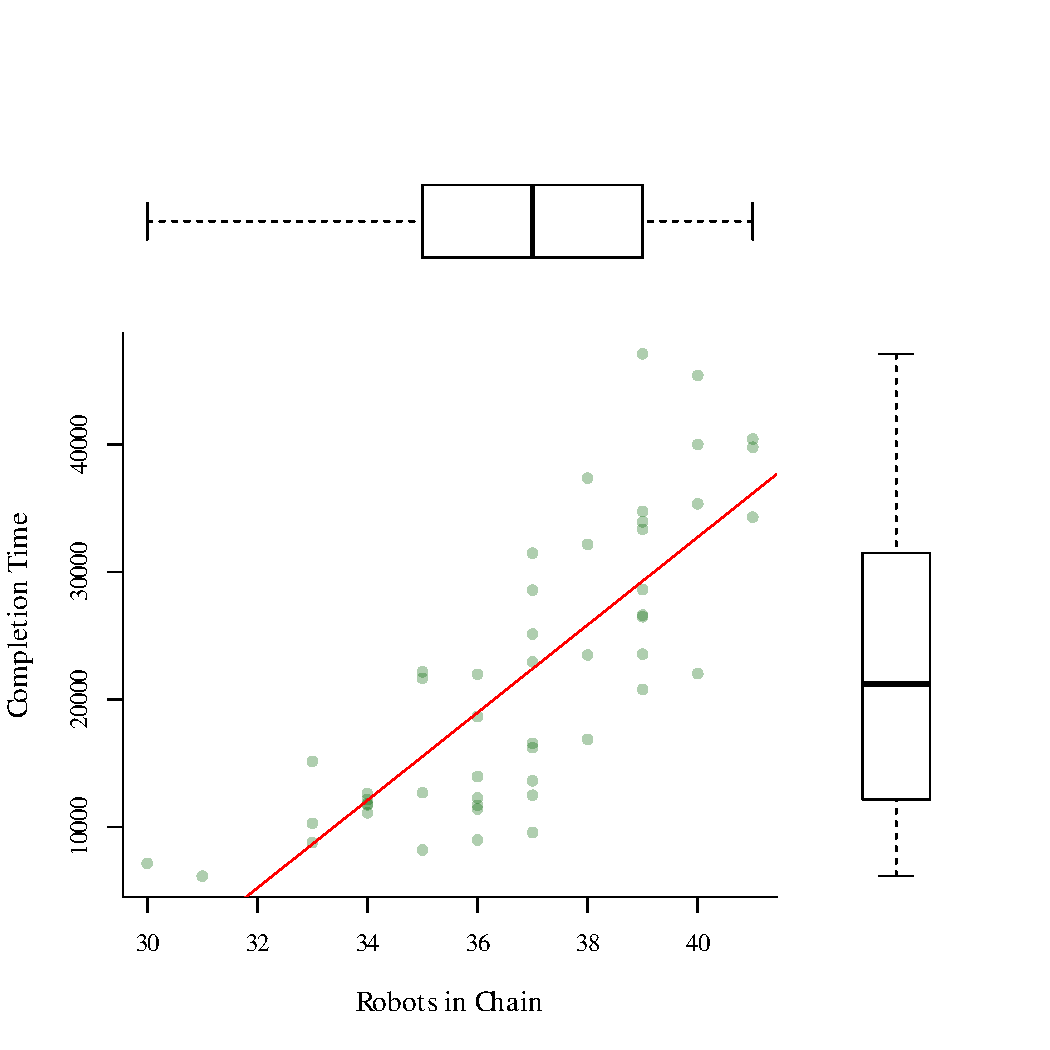
\includegraphics[width=\textwidth,keepaspectratio]{{../Results/50Trials/ResultsDistribution}.pdf}

(a)

\end{center}
\end{minipage}%
\hspace{0.5cm}
\begin{minipage}{.35\textwidth}
\begin{footnotesize}
\begin{center}

\begin{tabular}{|l|c|c|}
\hline
& \textbf{Value} & \textbf{P-Value} \\
\hline
\textbf{Pearson - } $\mathbf{r}$  &	0.7934599 & 6.357e-12 \\
\hline
\textbf{Kendall -} $\mathbf{\tau}$ & 0.6691023 & 5.554e-11 \\
\hline
\end{tabular}
\label{tab:correlation}
\vskip15pt
(b)
\vskip15pt

\end{center}
\end{footnotesize}
\end{minipage}
\captionof{figure}{Enhanced scatter plot of the completion times as a function of the number of robots (a), with the results of the correlation analysis (b)}
\end{center}

Intuitively, one may assume that the completion time is positively correlated with respect to the number of robots in chain (since more robots require more time to be deployed).

This intuition is confirmed by the graphical representation of the completion time as a function of the number of robots in the chain, along with the representation of a linear model fitting the points obtained through the experiment as well as by the values of the correlation coefficients, and their statistical significance (attested by a p-value considerably small than the confidence level $1-\alpha=0.05$.

\bibliographystyle{plain}
\bibliography{References}
